\paragraph{Autenticazione}

\label{Autenticazione}

\begin{figure}[ht]
	\centering
	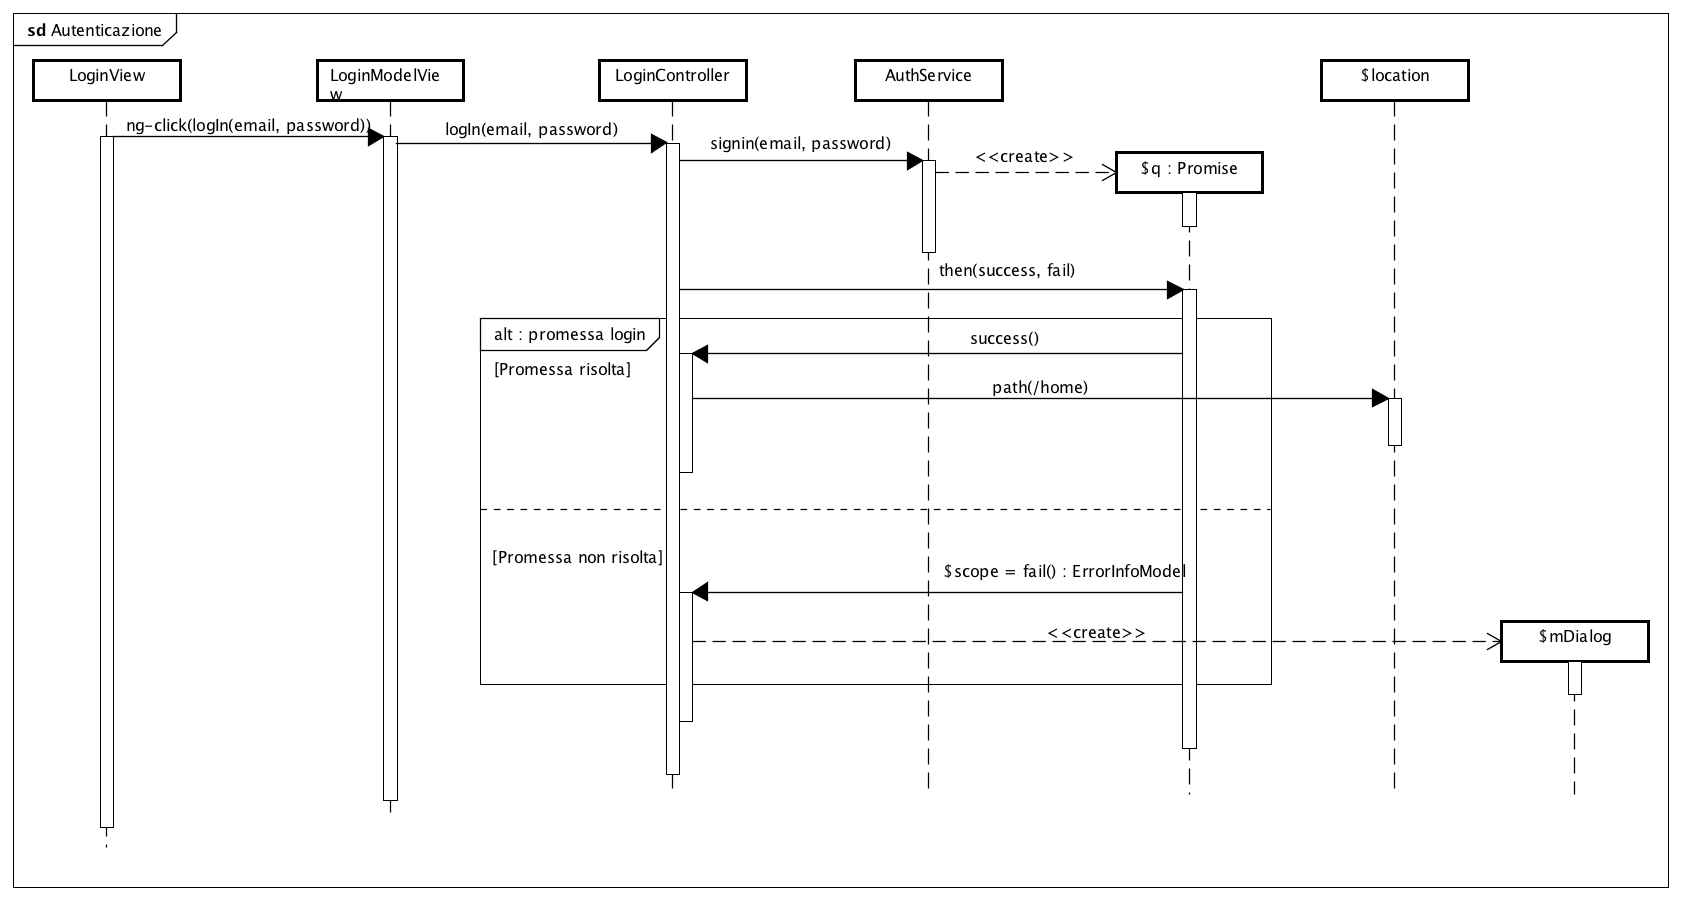
\includegraphics[scale=0.35,keepaspectratio]{UML/DiagrammiDiSequenza/Front-end/Login.png}
	\caption{Autenticazione}
\end{figure} \FloatBarrier

L'utente, dopo aver inserito i campi email e password, può effettuare l'autenticazione avviando l'evento associato al bottone presente in \texttt{LoginView}. Il \texttt{LoginController} gestisce l'evento chiamando il metodo \texttt{signin} dell'\texttt{AuthService}, il quale restituisce una promessa. Se la promessa è soddisfatta l'utente viene reindirizzato alla home page, altrimenti verrà restituito un oggetto di tipo \texttt{ErrorInfoModel} e mostrato a video mediante \texttt{\$mdDialog}.